\documentclass[12pt]{scrartcl}

\usepackage[american]{babel}

\usepackage{graphicx}
\graphicspath{{images/}}

\usepackage{paralist}
\usepackage{csquotes}
\usepackage[T1]{fontenc}
\usepackage{lmodern}
\usepackage[marginal]{footmisc}

\usepackage{geometry}
% \geometry{a4paper,body={5.8in,9in}}
\geometry{a4paper}

\usepackage{amsmath, amsfonts, amssymb}
\usepackage{placeins}
\usepackage{subcaption}

\usepackage{setspace}

\setlength{\parindent}{0pt}
%
%%%%%%%%%%%%%%%%%%%%%%%%%%%%%%%%%%%%%%
% ab hier steht der eigentliche Text:
\begin{document}

\title{Automatic Ranking of Classification Algorithms}
\subtitle{A Comparison of Regression-Based Ranking and Preference Models
\\\vspace{2em}Bachelor Thesis Proposal \& Work Plan}

\author{Helena Graf\\ 
\small{matriculation number: 7011643}\\ 
\small{hgraf@mail.upb.de}}
\date{\today}

\maketitle
\vspace{2em}

\begin{center}
\small{Supervisors:}\\
\large{Prof. Dr. Eyke H\"ullermeier}\\
\large{Prof. Dr. Axel-Cyrille Ngonga Ngomo}
\end{center}

\newpage
\tableofcontents
\newpage

\section{Motivation}\label{sec:motivation}

\section{Task Objectives}\label{sec:task-objectives}

\section{Task Description}\label{sec:task-description}

\newpage

\section{Initial Document Structure}\label{sec:doc-structure}
\begin{enumerate}
	\item Introduction
	\begin{enumerate}[1.1]
		\item Solution Approach
		\item Structure
	\end{enumerate}
	\item Fundamentals
	\begin{enumerate}[2.1]
		\item ML-Plan? weka? jpl?
		\item Ranking Algorithms
		\item Spearmans's Rank Correlation Coefficient
	\end{enumerate}
	\item Implementation
	\begin{enumerate} [3.1]
		\item Regression-based Ranking
		\begin{enumerate}[3.1.1]
			\item Static Algorithm
			\item Automatic Algorithm Selection
		\end{enumerate}
		\item Preference Models
	\end{enumerate}
	\item Evaluation
	\begin{enumerate}[4.1]
		\item Computing the Accuracy of the Results
		\item Assessment of Accuracy
	\end{enumerate}
	\item Related Work
	\begin{enumerate}[5.1]
		\item Evolutional Algorithms
		\item Runtime Predictions
	\end{enumerate}
	\item Conclusion
	\item Literature
	\item Appendix
\end{enumerate}

\newpage

\section{Time-Schedule and Subtasks}\label{sec:schedule-and-subtasks}

% % %
\begin{figure}[!ht]
	\centering
	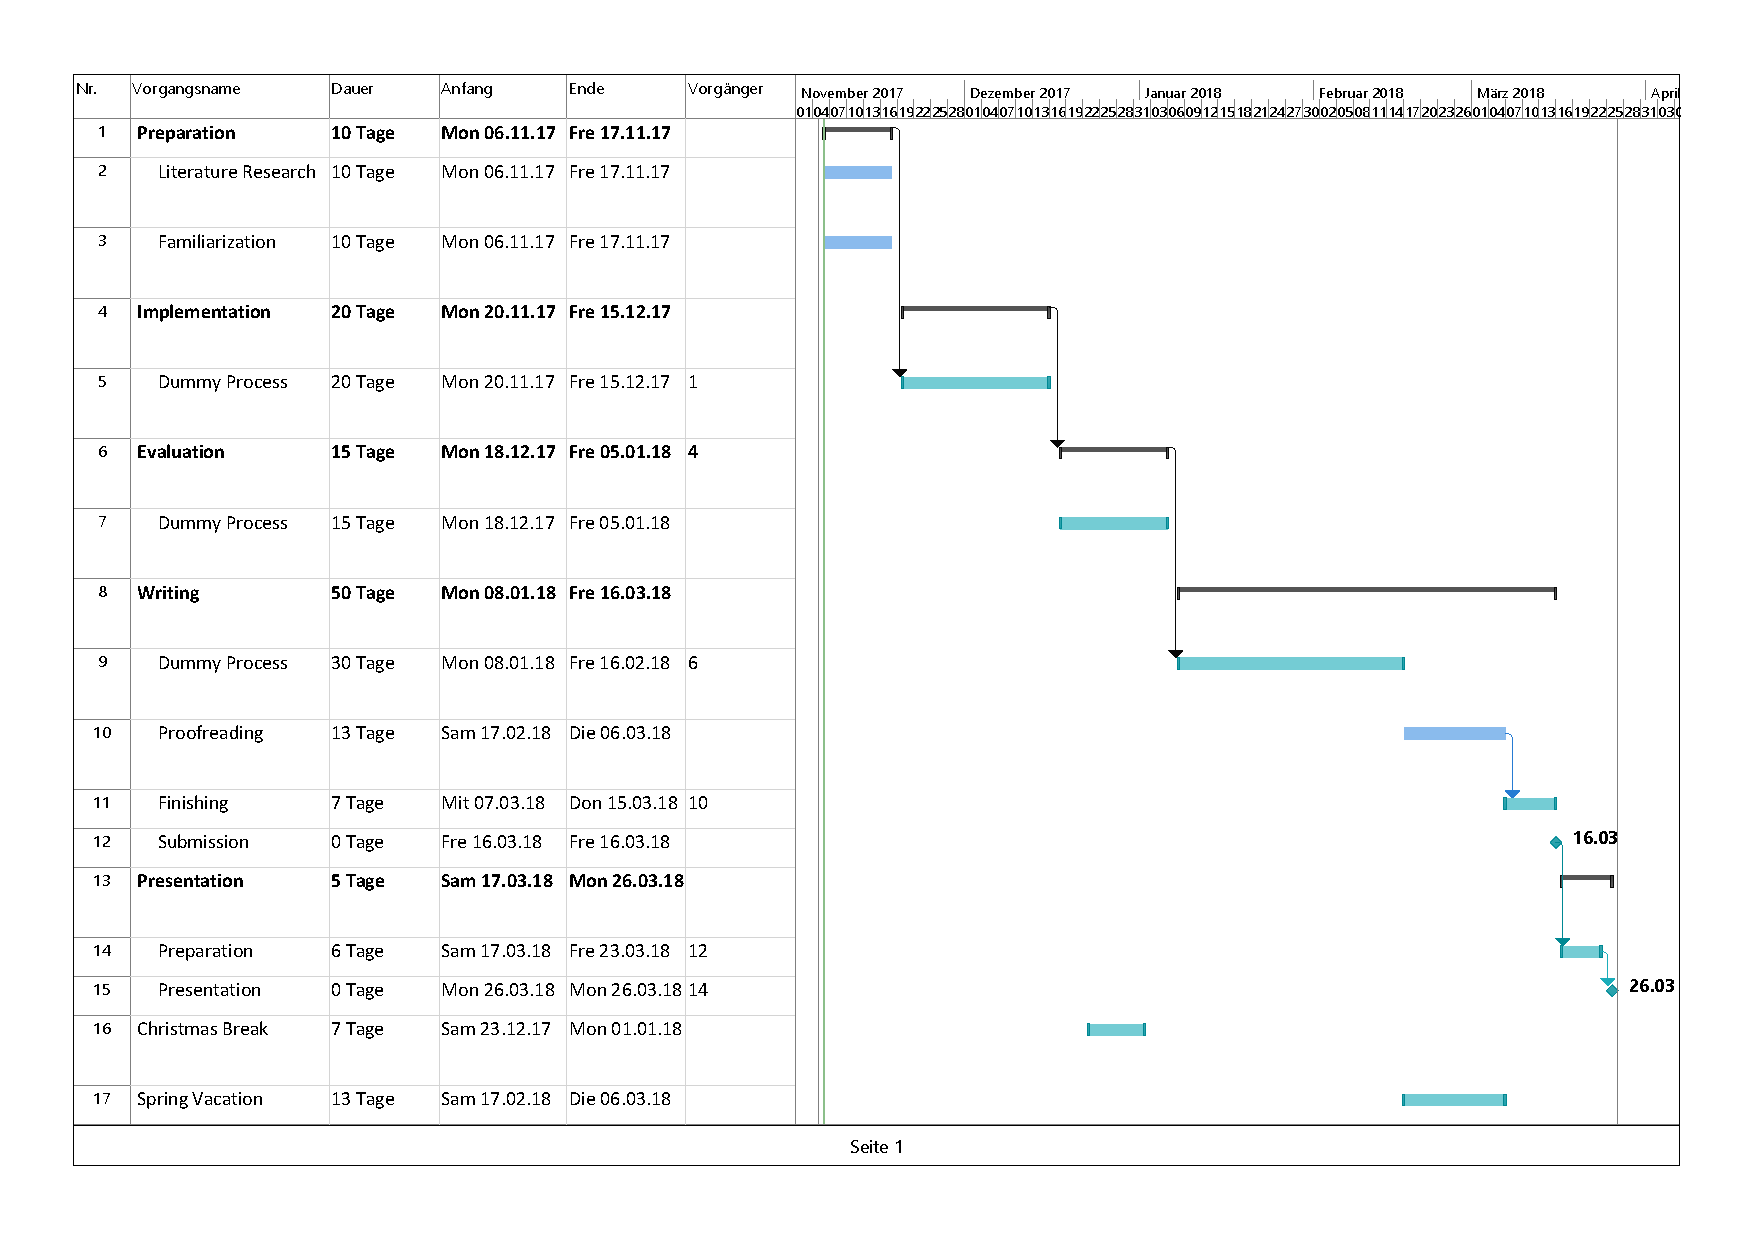
\includegraphics[width=.9\textwidth]{Gantt_BA_Helena}
	\caption{Sketch of the time schedule for the work on the thesis}
	\label{fig:time-schedule}
\end{figure}
% % %

\newpage

\bibliography{literature}
\bibliographystyle{myalphadin}

\vspace{6cm}

\begin{center}
     \begin{tabular}{l p{0.1\textwidth} r}
       \cline{1-1} \cline{3-3}
       \begin{minipage}[t]{0.4\textwidth}
         \centering
         Supervisor\\(Prof. Dr. Eyke H\"ullermeier)
         \end{minipage}
&
         \begin{minipage}[t]{0.2\textwidth}
         \end{minipage}
&
         \begin{minipage}[t]{0.4\textwidth}
           \centering
           Student\\(Helena Graf)
         \end{minipage}
     \end{tabular}
\end{center}

\end{document}
